\documentclass[sigconf]{acmart/acmart}
\usepackage{lipsum}

\AtBeginDocument{%
    \providecommand\BibTeX{{%
                Bib\TeX}}}

\begin{document}
\title{GAN Report Document}
\author{sailing-innocent}
\authornote{updated March 19th. 2023}
\email{some@email}

\affiliation{%
    \institution{Jialidun University}
    \streetaddress{Some Where on Earth}
    \city{The City}
    \state{The State}
    \country{The Country}
    \postcode{xxxxxx}
}
\begin{abstract}
    \lipsum[3]
\end{abstract}

\keywords{AIGC, Geometric Deep Learning, Terrain Generation, 3D Reconstruction, Multi-view Synthesis}
%% A "teaser" image appears between the author and affiliation
%% information and the body of the document, and typically spans the
%% page.
\begin{teaserfigure}
    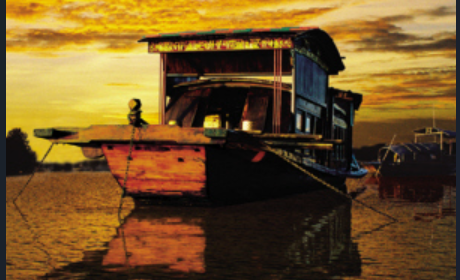
\includegraphics[width=\textwidth]{fig_boat.png}
    \caption{Boat}
    \Description{The Boat}
    \label{fig:teaser}
\end{teaserfigure}

\maketitle

\section{This is GAN}

\paragraph{GAN}

Generative Advesarial Network \cite{goodfellowGenerativeAdversarialNetworks2014}

\begin{figure}
    \centering
    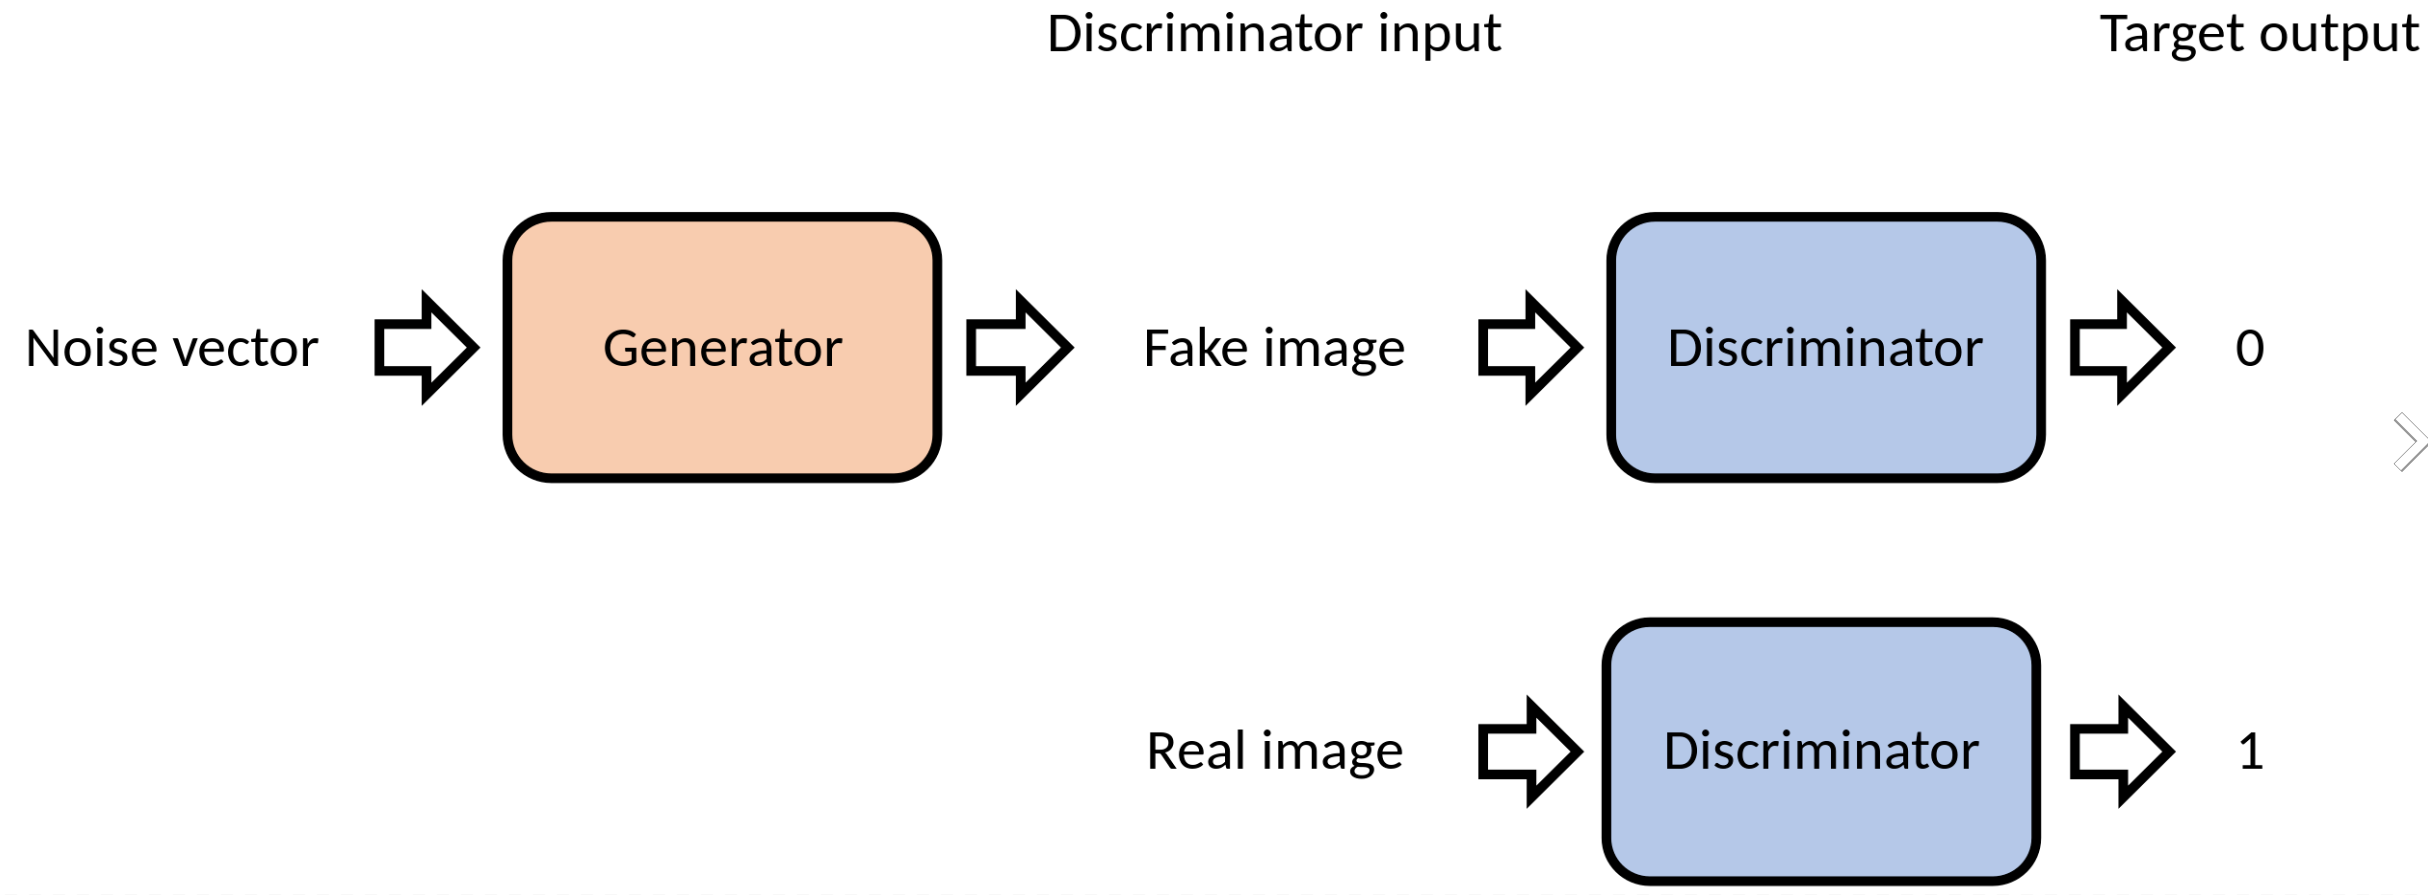
\includegraphics[width=\linewidth]{fig_gan_wiki.png}
    \caption{The GAN structure}
\end{figure}

\subparagraph{Brief}
Two MLPs were trained using back-propogation as
\begin{itemize}
    \item Generative Model G
    \item Discriminative Model D
\end{itemize}

The Generative Model captures data distribution.
The Discriminative Model estimates the probability that a sample is from trained data or not.

\textbf{Ideal Result}:
\begin{itemize}
    \item G could generate the data in trained set
    \item D equal to $\frac{1}{2}$ ( so that it cannot determine whether the generated data is from trained set or not)
\end{itemize}

And The Loss Function

$$\min_G\max_DV(D,G) = E_{x\sim p_{data}(x)}[logD(x)] + E_{z\sim p_{z}(z)}[log(1 - D(G(z)))]$$



\section{This is Diffusion}

\paragraph{Diffusion Model}

The Diffusion Model originates from DDPM \cite{hoDenoisingDiffusionProbabilistic2020}

\bibliographystyle{acmart/ACM-Reference-Format}
\bibliography{ref}
\end{document}
\endinput
